\documentclass[3p]{elsarticle}
%\documentclass[3p, twocolumn]{elsearticle}
\usepackage{amsmath}
\usepackage{amssymb}
\usepackage{gensymb}
\usepackage{upgreek}
\usepackage{float}
\parskip=0pt

\begin{document}

\begin{frontmatter}

\title{Resistance mapping of anti-corrosion polymer coatings using a scanning electrochemical microscope}
\cortext[cor]{Corresponding author}
\author[akiss]{Andr\'{a}s Kiss\corref{cor}}
\address[akiss, gnagy]{Department of General and Physical Chemistry, Faculty of Sciences, University of P\'{e}cs, 7624 P\'{e}cs, Ifj\'{u}s\'{a}g \'{u}tja 6, Hungary}
\address[akiss, gnagy]{J\'{a}nos Szent\'{a}gothai Research Centre, University of P\'{e}cs, 7624 P\'{e}cs, Ifj\'{u}s\'{a}g \'{u}tja 20, Hungary}
\ead{akiss@gamma.ttk.pte.hu}
\author[lkiss]{L\'{a}szl\'{o} Kiss}
\author[gnagy]{G\'{e}za Nagy}
\ead{g-nagy@gamma.ttk.pte.hu}

\begin{abstract}
A novel application of the scanning electrochemical microscope is presented, that allows mapping the resistance of an insulating layer on a conductive surface. Corrosion of coated iron is used as an example to investigate the efficiency of the technique. A thin carbon fiber was rastered on polypyrrole and polyphenol coated iron samples while maintaining direct contact between the tip of the carbon fiber and the studied surface. The potential of the carbon fiber was measured against the iron sample while it was immersed in a corrosive medium. Depending on the resistance between the tip and the sample, the measured voltage proportionally varied between 0 and the open circuit potential of the potentiometric circuit formed by the iron sample, the electrolyte and the carbon fiber. The resistance varies with spatial coordinates because of the buildup of the corrosion products and the inhomogeneity of the protective insulation. Using the voltage divider formula, a resistance map could be calculated from the measured potential map. Based on the obtained images, the quality of the coatings could be established, and weak spots could be identified.
\end{abstract}

\begin{keyword}
	scanning electrochemical microscope \sep corrosion product
\end{keyword}
\end{frontmatter}

\section{Introduction}
There are several efficient polymer coatings for corrosion protection of iron and its alloys. Among the most investigated polymers for this purpose are polypyrrole and polyaniline due to the relatively low oxidation potential of their monomers and because they form a compact and adherent layer on iron and many other metals and alloys. A huge number of works are describing the barrier properties of polypyrrole in different media like salt water and acidic solutions [1-6]. Multilayers like polyaniline-polypyrrole showed excellent protective characteristics compared to individual layers [7]. Polyphenols can also build up adherent coatings on surfaces of steel alloys but they are less investigated than the above mentioned polymers. Natural polyphenols proved themselves to be good adsorption inhibitors of carbon steel at lower temperatures [8-11]. On galvannealed iron, the polyphenol layer can be impregnated with manganese sulfate, manganese phosphate and polyethylene wax to improve corrosion resistance [12]. Different polyphenols can be electrodeposited from phenol and from its monosubstituted derivatives, because they quickly foul  metal substrates, and have corrosion protection properties [13-16].

Methods for coating the metal substrate by electrooxidation are usually cyclic voltammetry, galvanostatic and chronopotentiometric deposition. In the deposition solution, the presence of additives such as tartrate contributes to the formation of adherent and protective layers on the substrate surface [17].

The investigation of anti-corrosion coatings is important. In this work we use anti-corrosion coatings as examples to evaluate the performance of a new surface resistance mapping electrochemical method. The technique is based on mapping the potential of the studied surface, and then calculating the resistance map from those values using the voltage divider equation. It must be mentioned, that a similar technique has already been worked out to map potential distributions in functioning silicon devices. The technique uses an atomic force microscope with a conductive cantilever. It was originally called nanopotentiometry 

[Trenkler T, De Wolf P, Snauwaert J, Qamhieh Z, Vandervorst W, Hellemans L. Local potential measurements in silicon devices using atomic force microscopy with conductive tips. In Solid State Device Research Conference, 1995. ESSDERC'95. Proceedings of the 25th European 1995 Sep 25 (pp. 477-481). IEEE.

,

Trenkler T, De Wolf P, Vandervorst W, Hellemans L. Nanopotentiometry: Local potential measurements in complementary metal–oxide–semiconductor transistors using atomic force microscopy. Journal of Vacuum Science & Technology B: Microelectronics and Nanometer Structures Processing, Measurement, and Phenomena. 1998 Jan;16(1):367-72.],


and later scanning voltage microscopy


[Ban D, Sargent EH, Dixon-Warren SJ, Calder I, SpringThorpe AJ, Dworschak R, Este G, White JK. Direct imaging of the depletion region of an InP p–n junction under bias using scanning voltage microscopy. Applied physics letters. 2002 Dec 23;81(26):5057-9.]. 


The performance of the proposed method was investigated through the example of mapping the resistance of two widely used and well known organic anti-corrosion coatings, polypyrrole and polyphenol.

\section{Experimental}
The surface of epoxy (epofix?) embedded disc shaped carbon steel [target preparation method paper] sample was sanded off on a 2000 grid emery paper to remove the holes and locally corroded areas from the metal sample. Then, the substrate was thoroughly washed with tap water to avoid the formation of scratches during the subsequent mirror finishing step where the metal surface was made flat and smooth with polishing with a 4000 grid emery paper. After thorough washing with tap water and deionized water the substrate was allowed to dry.
For making the coatings 0.1 M potassium sodium tartrate (Reanal, Hungary) was dissolved in deionized water (k <= 2 uS/cm), which is necessary to improve the adherence of the polymer layer. The corresponding monomer (pyrrole or phenol, products of Reanal, Hungary) was also dissolved in 0.5 M concentration in this solution. The counter electrode was a d = 1.6 mm, l = 7 cm rod made of titanium and coated with platinum (eDAQ, Australia), a standard calomel (SCE) served as reference electrode.

(The adherence of the coating might be influenced by the technique used for the deposition.) A small container was formed above the mould by wrapping the sides with sellotape to create walls. 2 ml of the monomer containing solution was put in the formed container and chronopotentiometry was used for the deposition process by setting 5 mA/cm^2 (31 A on 0.62 mm^2) constant current density and 30 s running time. Fig. 1 shows the recorded chronopotentiometric curve for the electrodeposition processes. It can be seen that initially the cell voltages are low due to the dissolution of metal when making both types of organic coatings but in time the voltages increase continuously caused by formation of a resistive layer composed of iron oxides and tartrate. After 3 s in presence of pyrrole monomer (curve a) a sharp and significant increase in the voltage could be observed which is attributable to the formation of highly resistive protective layers.

Curve b is related to the electrodeposition of phenol and it can be seen that the formed polyphenol film is less adherent than polypyrrole. The samples were washed thoroughly with deionized water to remove any monomer or tartrate residue. Bare iron was partially exposed under both layers by scratching them with a sharp medical needle to simulate damage. 2 ml of the 10^-3 M NaCl corrosive electrolyte was put into the sample container. The samples were left in the corrosive electrolyte for 30 minutes, after which scanning with the carbon fiber was started in the same solution. First, the fiber was centered above the coated sample (X = 0 um, Y = 0 um) at about 200 um height. The carbon fiber was moved down until it touched the surface, and then an additional 300 um to let it bend. The thickness of the polymer layers was smaller than 300 um, therefore the carbon fiber was pressed against the sample with a constant force.  Then, it was moved to the starting position of the scan at the coordinate X = -2000 um, Y = -2000 um. In this way, the entire sample was well within the borders of the 4000 um by 4000 um sized image. Unidirectional scanning had to be used to avoid the shift between the scan lines caused by the bend in the carbon fiber. The so-called “fast comb” scanning algorithm was used [scanning algorithm cikk]. A translation speed of 500 um/s was used between the adjacent data acquisition points. Step size in both axes was 100 um, resulting in 41x41=1681 data acquisition points. 0.3 s was allowed at each point to let the potentiometric measuring circuit reach a potential close to the equilibrium. In this way, 0.5 s was allocated to every point, since translation took 0.2 s between adjacent points. After obtaining the potential map, the resistance of the potentiometric circuit was measured by introducing a 100 kOhm precision resistor R3 between the carbon fiber and the iron sample. This formed an additional voltage divider with the resistance of the potentiometric circuit, R2 and E, the potential difference when R1 was very large compared to R2. The potential difference was measured before and after R3 was introduced into the circuit. Both measurements were performed three times, with the tip of the carbon fiber at three different locations with X,Y,Z coordinates (0,0,100), (0,0,500) and (-2000, -2000, 100) measured in um. The purpose of measuring at three different coordinates is to prove that the varying resistance of the electrolyte associated with different coordinates has little influence on the measured voltage V. Then, R2 was calculated with the voltage divider formula. After obtaining R2, R1 for every point was calculated by using the voltage divider formula again on every point of the measured potential map.

\section{Results and Discussion}
The proposed technique is based on rastering the carbon fiber in direct contact with the investigated surface, while measuring the potential of the fiber. The conductive sample, the non-conductive surface layer, the solution and the carbon fiber together form a voltage divider circuit as shown in Fig. 2.

The potential difference “V” is measured between the iron sample and the carbon fiber. When the carbon fiber does not touch the iron surface or even the polymer layer on top of it, and is only coupled to it through the electrolyte with resistance R2, the measured potential difference V will equal to “E”. However, when the carbon fiber is in contact with the bare iron sample surface, the potentiometric circuit is short circuited through the direct contact between the carbon fiber and the iron sample, and V=0. If the carbon fiber contacts an insulating layer between the iron sample and the carbon fiber, denoted by a resistance R1, the measured voltage is determined by the ratio of R1 and R2, according to the voltage divider formula:
If R2, E and V is known, R1 for every point can be calculated. R2 is the the resistance of the potentiometric circuit, which comes mostly from the electrolyte. It can be measured by using a precision resistor R3 to connect the lead of the carbon fiber and the lead of the iron sample. Then, if V is measured with and without R3 present in the circuit, R2 can be obtained by using the voltage divider formula, in this case:

Where V and E are the measured potentials with, and without the R3 shunt resistor in the circuit.



\begin{figure}[H]
\centering
% trim = top left bottom right
\includegraphics[trim = 15mm 30mm 0mm 15mm, clip, width=0.3\textwidth, angle=-90]{17052401.eps} 
\includegraphics[trim = 15mm 30mm 0mm 15mm, clip, width=0.3\textwidth, angle=-90]{17052402.eps}
\includegraphics[trim = 15mm 30mm 0mm 15mm, clip, width=0.3\textwidth, angle=-90]{17052403.eps} 
\includegraphics[trim = 15mm 30mm 0mm 15mm, clip, width=0.3\textwidth, angle=-90]{17052405.eps}
%\includegraphics[trim = 20mm 30mm 0mm 20mm, clip, width=0.3\textwidth, angle=-90]{18011710.eps} 

% trim = left bottom right top
%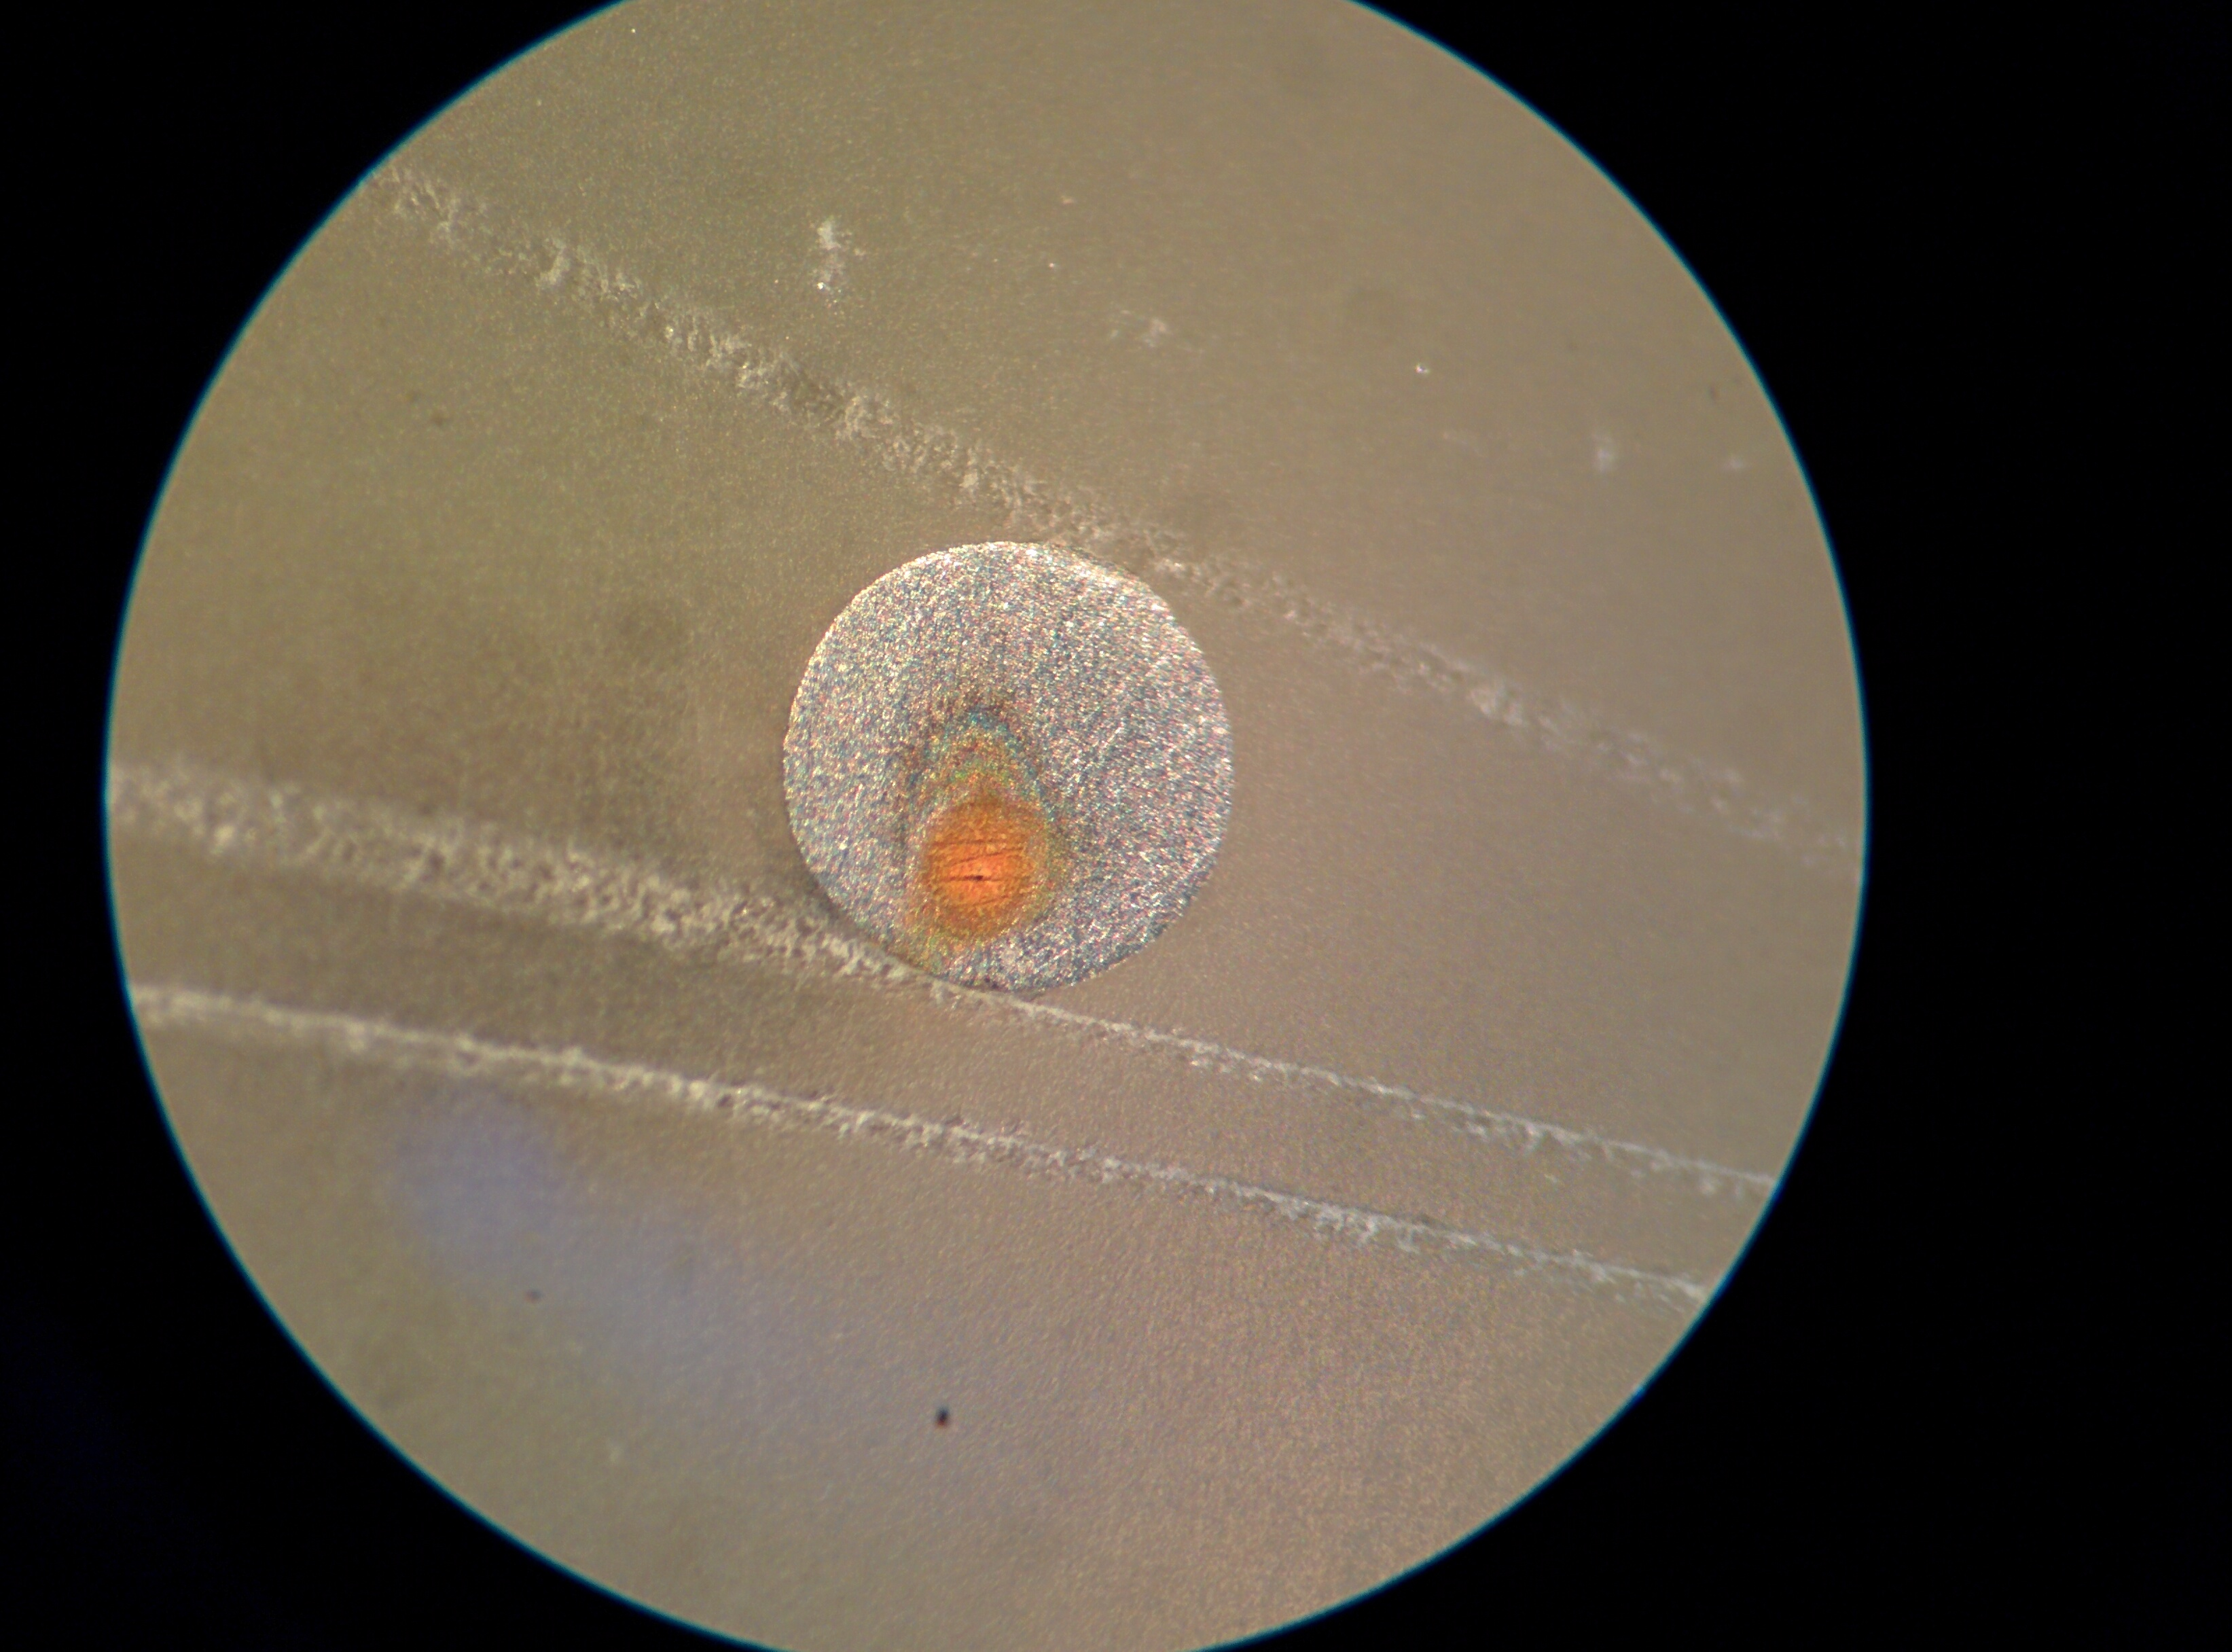
\includegraphics[trim = 350mm 300mm 460mm 250mm, clip, width=0.25\textwidth]{IMG.jpg}
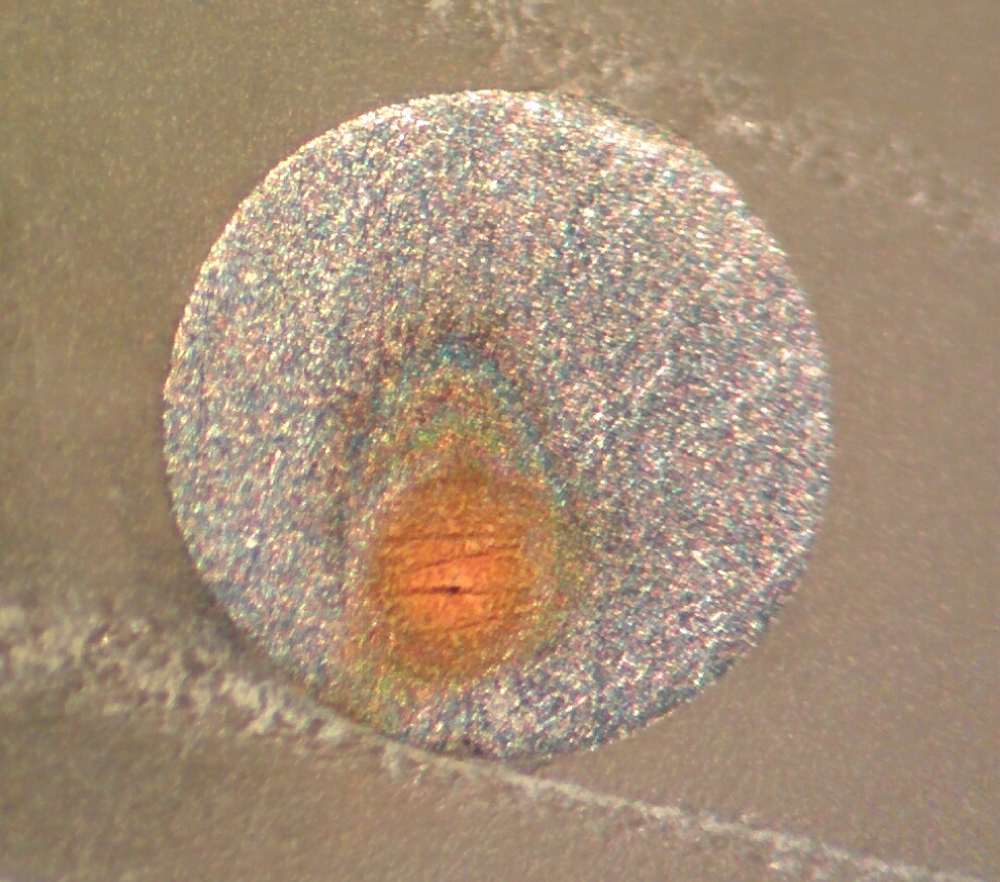
\includegraphics[width=0.25\textwidth]{img1.png}
\hspace{2cm}
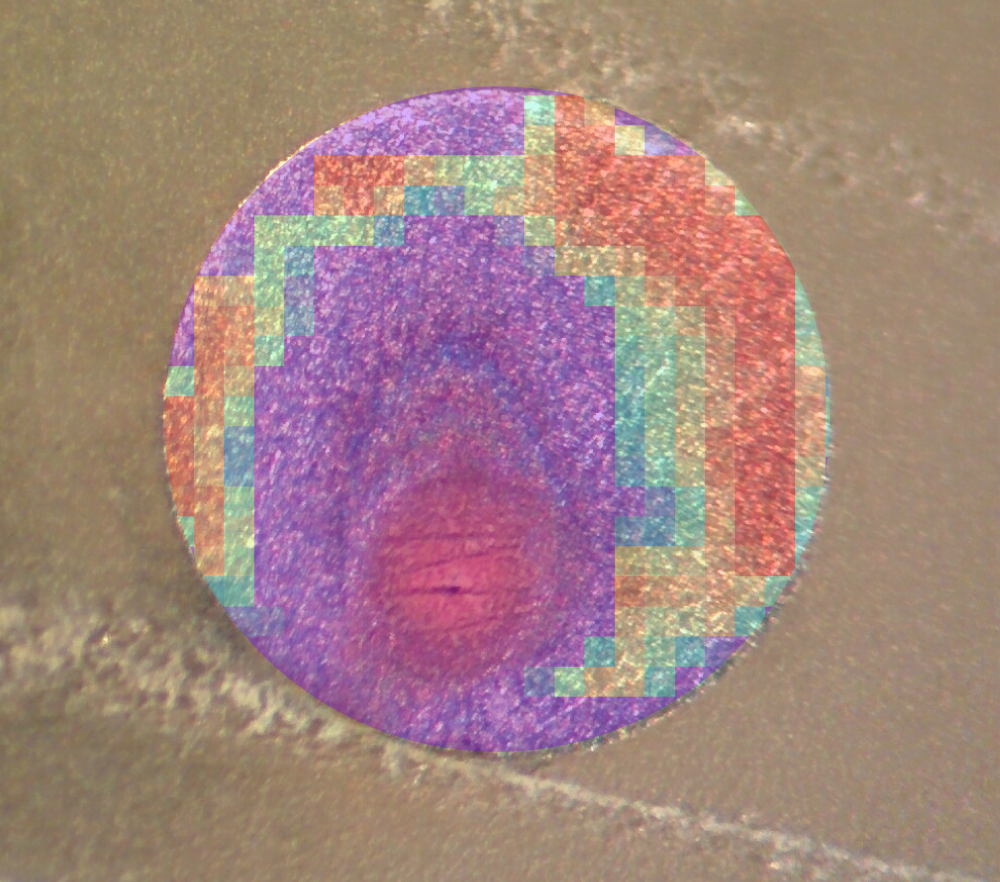
\includegraphics[width=0.25\textwidth]{img2.png}

\caption{Figure caption.}
\label{fig:deconvolution}
\end{figure}


%\begin{figure}[H]
%\centering
%% trim = top left bottom right
%\includegraphics[trim = 20mm 30mm 0mm 20mm, clip, width=0.3\textwidth, angle=-90]{18011710.eps} 
%\includegraphics[trim = 20mm 30mm 0mm 20mm, clip, width=0.3\textwidth, angle=-90]{18011711.eps}
%\includegraphics[trim = 20mm 30mm 0mm 20mm, clip, width=0.3\textwidth, angle=-90]{18011712.eps} 
%\includegraphics[trim = 20mm 30mm 0mm 20mm, clip, width=0.3\textwidth, angle=-90]{18011713.eps}
%\includegraphics[trim = 20mm 30mm 0mm 20mm, clip, width=0.3\textwidth, angle=-90]{18011714.eps} 
%\includegraphics[trim = 20mm 30mm 0mm 20mm, clip, width=0.3\textwidth, angle=-90]{18011715.eps} 
%\includegraphics[trim = 20mm 30mm 0mm 20mm, clip, width=0.3\textwidth, angle=-90]{18011716.eps} 
%\includegraphics[trim = 20mm 30mm 0mm 20mm, clip, width=0.3\textwidth, angle=-90]{18011719.eps} 
%\caption{Half covered.}
%\label{fig:deconvolution}
%\end{figure}

%\begin{figure}[H]
%\centering
%% trim = top left bottom right
%\includegraphics[trim = 20mm 30mm 0mm 20mm, clip, width=0.3\textwidth, angle=-90]{18011701.eps}
%\includegraphics[trim = 20mm 30mm 0mm 20mm, clip, width=0.3\textwidth, angle=-90]{18011702.eps}
%\includegraphics[trim = 20mm 30mm 0mm 20mm, clip, width=0.3\textwidth, angle=-90]{18011703.eps} 
%\includegraphics[trim = 20mm 30mm 0mm 20mm, clip, width=0.3\textwidth, angle=-90]{18011704.eps}
%\includegraphics[trim = 20mm 30mm 0mm 20mm, clip, width=0.3\textwidth, angle=-90]{18011705.eps} 
%\includegraphics[trim = 20mm 30mm 0mm 20mm, clip, width=0.3\textwidth, angle=-90]{18011706.eps} 
%\includegraphics[trim = 20mm 30mm 0mm 20mm, clip, width=0.3\textwidth, angle=-90]{18011707.eps} 
%\includegraphics[trim = 20mm 30mm 0mm 20mm, clip, width=0.3\textwidth, angle=-90]{18011708.eps}
%\caption{Fully covered.}
%\label{fig:deconvolution}
%\end{figure}

\begin{figure}[H]
\centering
% trim = top left bottom right
\includegraphics[trim = 15mm 30mm 0mm 15mm, clip, width=0.3\textwidth, angle=-90]{18012501.eps}\includegraphics[trim = 15mm 30mm 0mm 15mm, clip, width=0.3\textwidth, angle=-90]{18012406.eps}
\includegraphics[trim = 15mm 30mm 0mm 15mm, clip, width=0.3\textwidth, angle=-90]{18012501_deconvoluted.eps}\includegraphics[trim = 15mm 30mm 0mm 15mm, clip, width=0.3\textwidth, angle=-90]{18012406_deconvoluted.eps}
%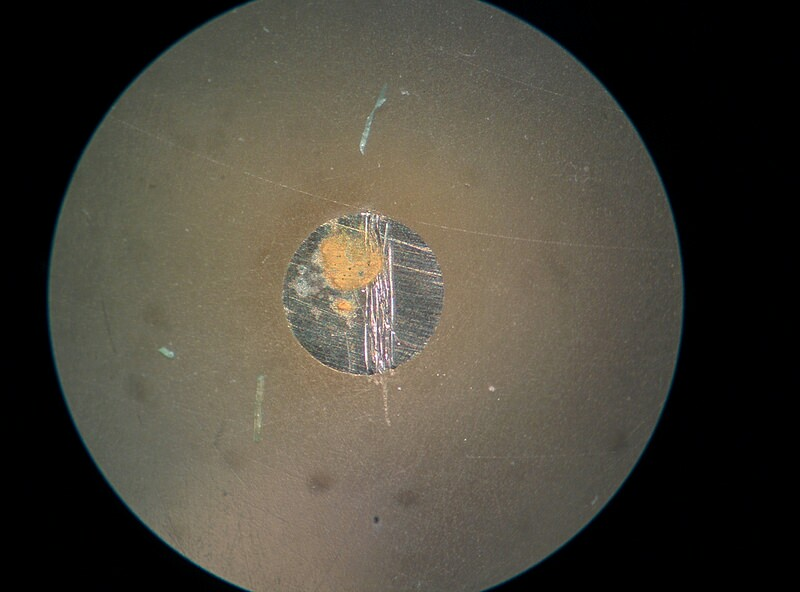
\includegraphics[trim = 350mm 300mm 460mm 250mm, clip, width=0.5\textwidth]{img.jpg}
% trim = left bottom right top
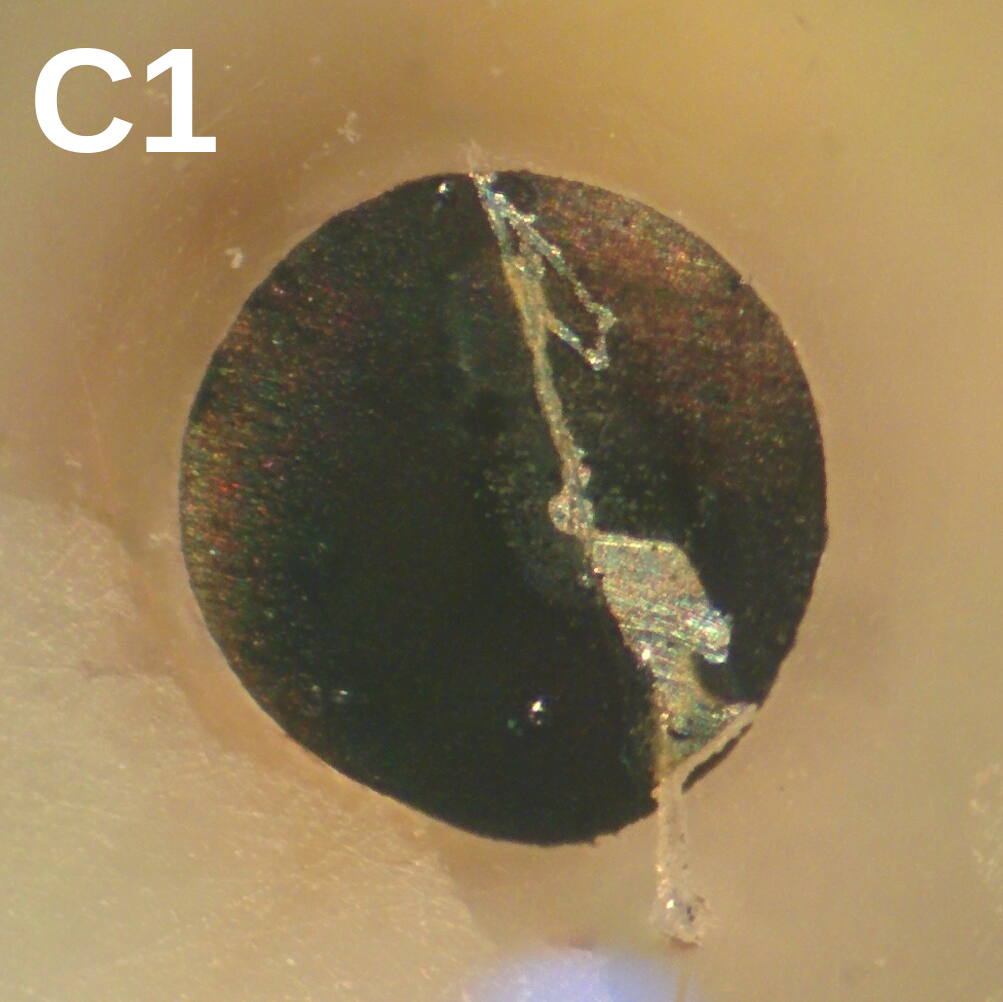
\includegraphics[width=0.25\textwidth]{ppyrrole_cut.jpg}\hspace{2cm}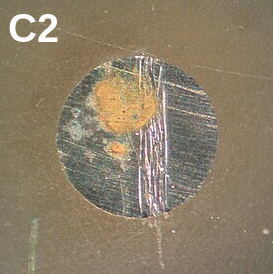
\includegraphics[width=0.25\textwidth]{pphenol_cut.jpg}
\caption{Polypyrrole.}
\label{fig:deconvolution}
\end{figure}

\begin{figure}[H]
\centering
% trim = top left bottom right
% trim = left bottom right top
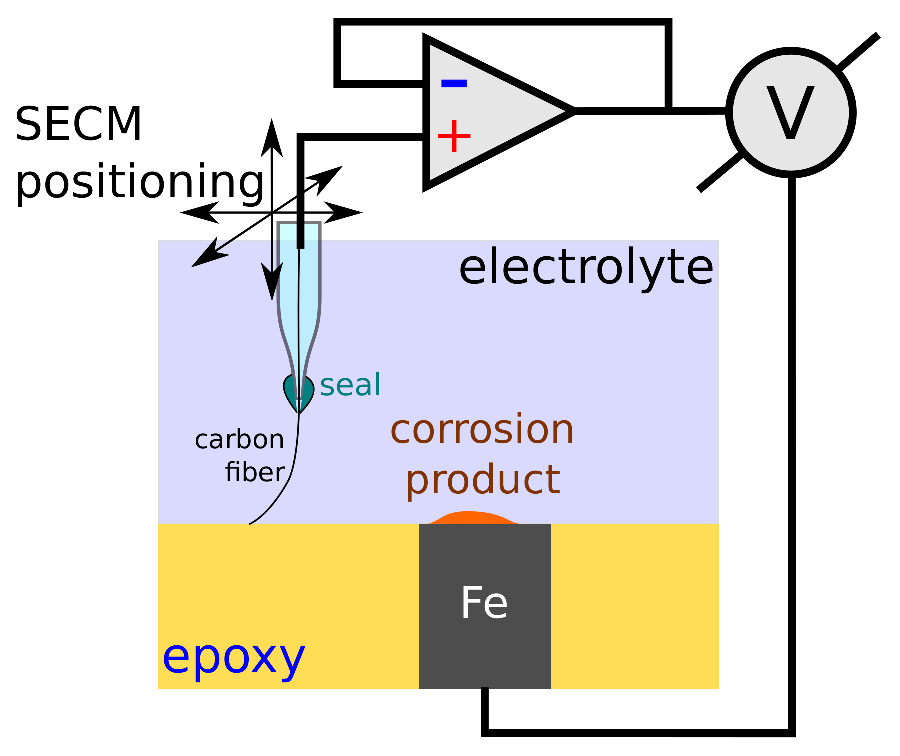
\includegraphics[width=0.6\textwidth]{whisker.eps}
%\includegraphics[trim = 20mm 30mm 0mm 20mm, clip, width=0.3\textwidth, angle=-90]{13121223.eps} 
\caption{Figure caption.}
\label{fig:deconvolution}
\end{figure}

\end{document}
